\chapter{Event Simluation and Object Reconstruction}\label{chapter:data-mc}
Following the readout of triggered events from the CMS detector, the reconstruction of the physics objects produced by the proton-proton collision is performed, allowing for the analysis of the underlying physical processes.
Monte Carlo (MC) simulations which provide a detailed, precise and realistic description of the expected SM and potential BSM processes at the LHC form an essential component of performing any analysis, allowing for the development of strategies to extract processes of interest from backgrounds and the ability to make statistical interpretations of the results, such as measuring and comparing the cross sections and other properties of a measured processes to theory or by setting limits on unobserved SM or predicted BSM processes.
The event simulation and objection reconstruction algorithms which are relevant to the single top physics search presented in this thesis are discussed in this chapter.

\section{Event Simulation}\label{sec:sim}
As MC simulation is meant to provide a realistic description of the expected SM and predicted BSM processes at the LHC, 
both accurate modelling of these processes and a detailed understanding of how physical processes interact with the CMS detector are required to produce events in the same format as raw proton-proton collision data prior to undergoing the same reconstruction process.
The simulation of events is a four stage process: generation (GEN), simulation (SIM), digitisation (DIGI) and reconstruction (RECO).

The initial GEN stage involves the use \emph{event generators} to simulate the proton-proton interactions and the resultant physics processes~\cite{Buckley:2011ms,Hoche:2014rga}.
The first stage of this is the modelling of the colliding protons and the hard scattering of their constituent partons, which involves the use Parton Distribution Functions (PDFs) to assign fractions of the protons momentum to the partons and perturbation theory to compute the matrix elements of the QCD and electroweak processes involved.
The second stage models resultant parton showers through an iterative process until the infrared cutoff scale for the shower is reached, with the remaining particles undergoing hadronisation.
The various event generators used in the production of MC samples used in this thesis are discussed in~\ref{subsec:eventGenerators}.

Following the GEN stage, the SIM stage involves passing the GEN output through a complete simulation of the CMS detector that has been with the GEANT4 program~\cite{geant4,Lefebure:1999wja}.
This process models particle interactions and decays and the propagation of particles through the detector, the effects of solenoidal field and detector material.
The DIGI stage uses the SIM output to produce the detector's electronics response, which then undergoes the same RECO process that data does, as described in~\ref{sec:reco}.

The inelastic proton-proton interactions, typically called pileup (\PU), which occur both within and adjacent to the event's bunch crossing, referred to as \emph{in-time} and \emph{out-of-time] \PU  respectively, also require modelling in simulation.
Simulated \PU however, does not adequately describe observed \PU in data.
Therefore, the reweighting of the simulated samples is required and is discussed in~\ref{}.
\editComment{insert ref or discuss in this chapter rather than in the analysis chapter?}.

\subsection{Event Generators}\label{subsec:eventGenerators}
\paragraph{aMC@NLO}
aMC@NLO~\cite{Alwall:2014hca} is a package that simulates processes to Next-To-Leading (NLO) order through the use of tree-level and one-loop
\paragraph{Madgraph}
\paragraph{POWHEG}
\paragraph{Pythia}

\section{Object Reconstruction}\label{sec:reco}
Using the readouts of all of the CMS sub-detectors, a full reconstruction of the triggered physics event is undertaken.
This process involves the \emph{Particle Flow} (PF) algorithm~\cite{CMS:2009nxa,CMS:2010eua,CMS-PRF-14-001} combining the physics objects constructed by sub-detectors to reconstruct and identify all the stable particles present in the event, such as electrons, muons, photos and neutral and charged hadrons and from these objects, higher-level objects such as jets, b-jets and missing transverse momentum can be constructed.

\subsection{Particle-Flow}

\subsection{Physics Object Reconstruction}
\subsubsection{Tracks and Primary Vertices}
\subsubsection{Electrons}
Electrons 
\subsubsection{Muons}
\subsubsection{Lepton Isolation}
The relative isolation of a lepton 
\subsubsection{Jets}
Due to colour confinement, quarks and gluons produced from the proton-proton hard interaction rapidly hadronise, producing a collimated shower of hadrons known as a \emph{jet}~\cite{Salam:2009jx}.
The \emph{anti-\kt} algorithm is used by CMS to ... in an infrared and collinear safe 
,Cacciari:2008gp

\subsubsection{b-Jets}
Correctly determining whether or not a jet was the product of a bottom quark hadronising is incredibly important for a variety of analyses, allowing them to separate signal processes from topologically similar background processes, including top physics searches due to the top quark's branching ratio to a W boson and bottom quark being $> 99\%$.
Such identification, known as \emph{b-taggging}, exploits the fact that due b hadrons having a relatively long lifetime of $\approx 1.5 ps$~\cite{Beringer:1900zz}, they travel a measurable distance away from the primary vertex before decaying. 
These secondary vertices are exploited by the \emph{Combined Secondary Vertex version 2} (CSVv2) algorithm~\cite{Chatrchyan:2012jua,CMS:206kkf}, which uses information about displaced track and secondary vertices as input into a multilayer perceptron ~\footnote{A class of neural network} to produce a discriminator value.
The CMS B-Tag and Vertexing (BTV) Physics Object Group defines working points for this (and other) algorithm's discriminator based on the mis-identification rate.

\editComment{insert fig re. discriminator}
\begin{figure}[h]
\centering
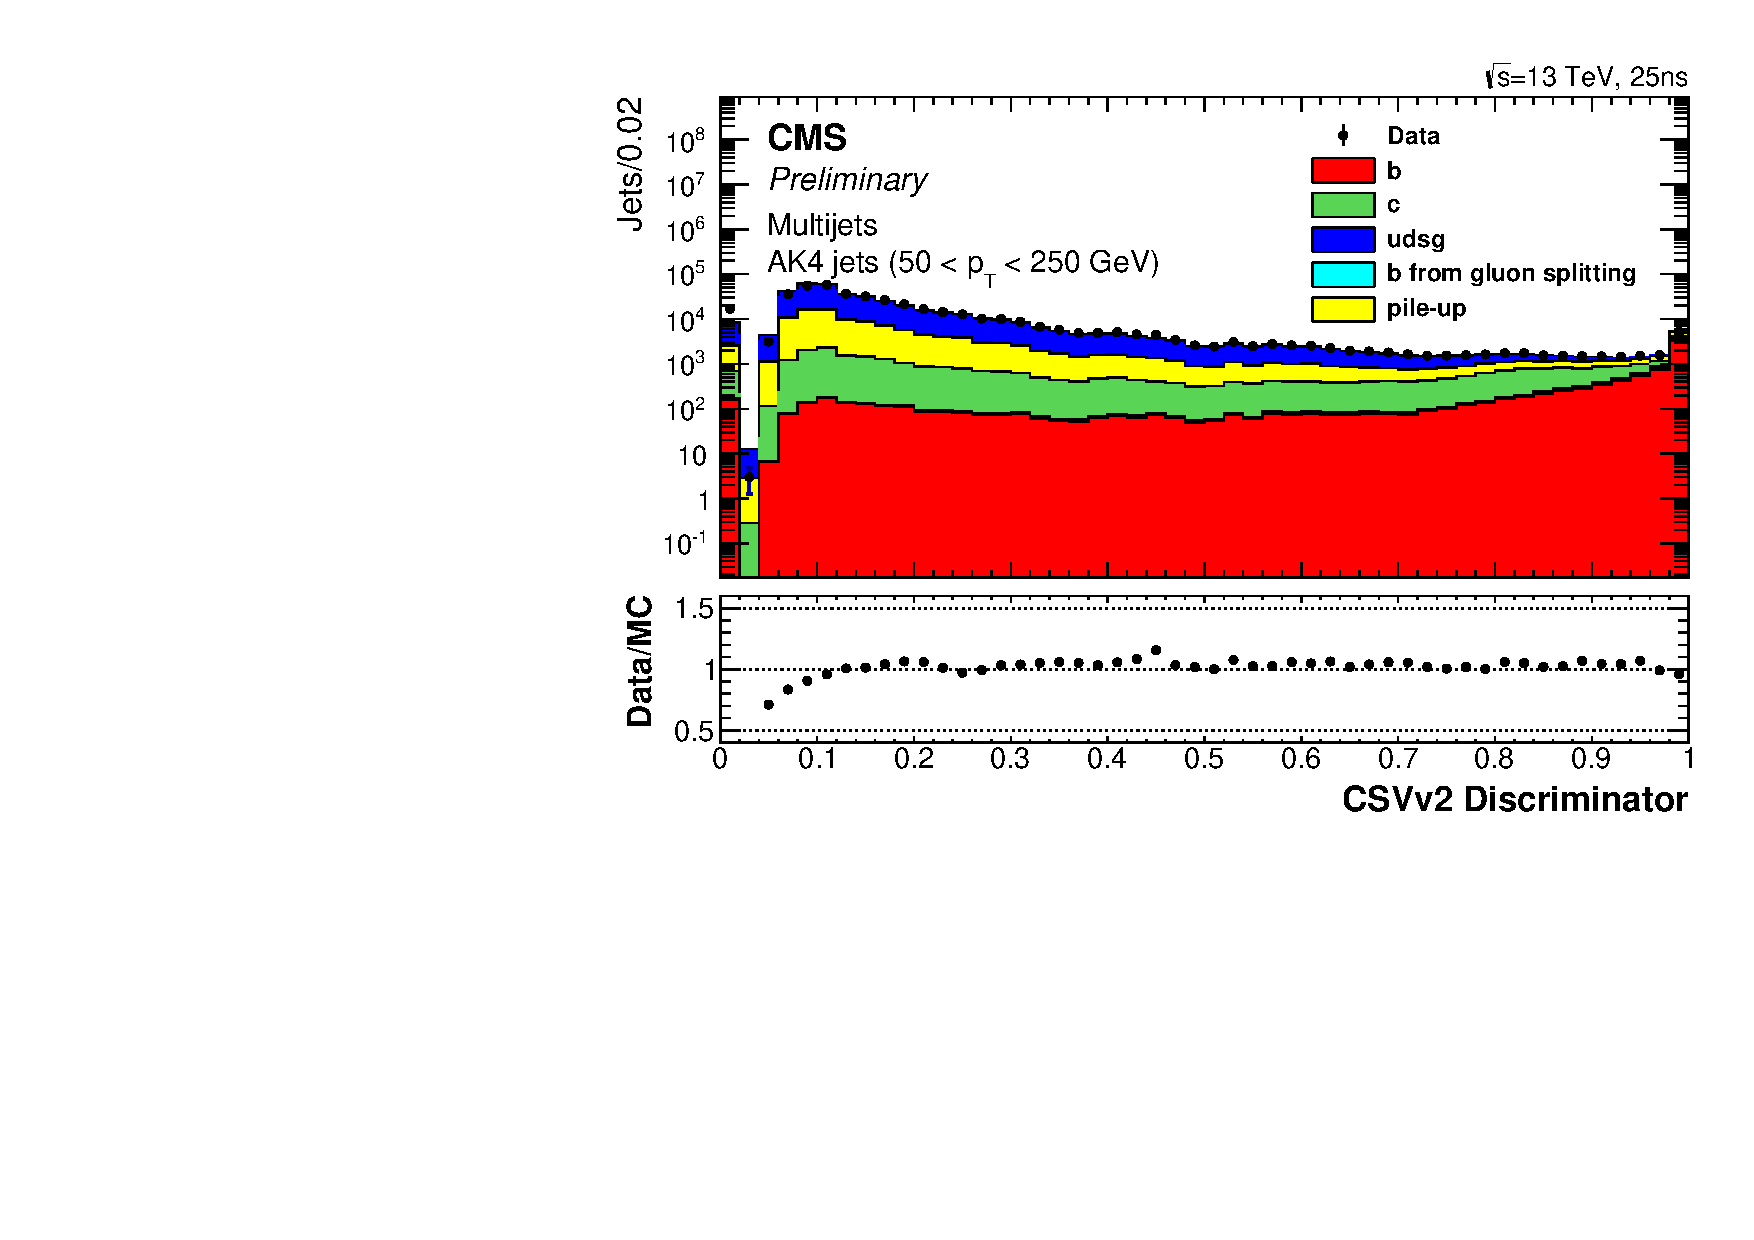
\includegraphics{figs/data-mc/ak4_pfjets_CSVIVF_Log.pdf}
\caption{The distribution of the CSVv2 algorithm's discriminator for multijet events, for $50\GeV < \pT < 250\GeV$, at \sqrt{13\TeV, where the jets have been reconstructed with the anti-\kt algorithm with R = 0.4~\cite{CMS:2016kkf}.}
\label{fig:bTagDiscriminator}
\end{figure}

\subsubsection{Missing Transverse Energy}
Particles which only weakly interact with matter, such as neutrinos and some hypothesised BSM particles, escape the detector without being directly observed, but can be inferred from considering the conservation of the transverse momentum of the event.
Therefore, the missing energy in the plane transverse to the beam line, \overrightarrow{\MET}, is defined as the negative vector sum of the transverse momentum in the end:

\begin{equation}
\overrightarrow{\MET} = - \sum \overrightarrow{\pT}\;.
\label{eq:MET}
\end{equation}

There are several different algorithms, using differing variables and techniques, which are used in CMS analyses to determine \MET.
PF \MET, producing using the PF particles, is used in this analysis because of its high performance with \emph{Type-I} \MET corrections applied~\cite{CMS:2016ljj}.
This correction applies the jet energy corrections discussed in~\ref{} to the PF jets with $\pT >15\GeV$ which are used in calculating the \MET.
Given that the event selection for the analysis presented in this thesis uses jets with $\pT > 30\GeV$, the \emph{Type-II} corrections (discussed in detail in~\cite{Chatrchyan:2011tn}) applied to jets with $\pT < 15\GeV$ is not considered.